\begin{figure*}[t]%
	\centering
	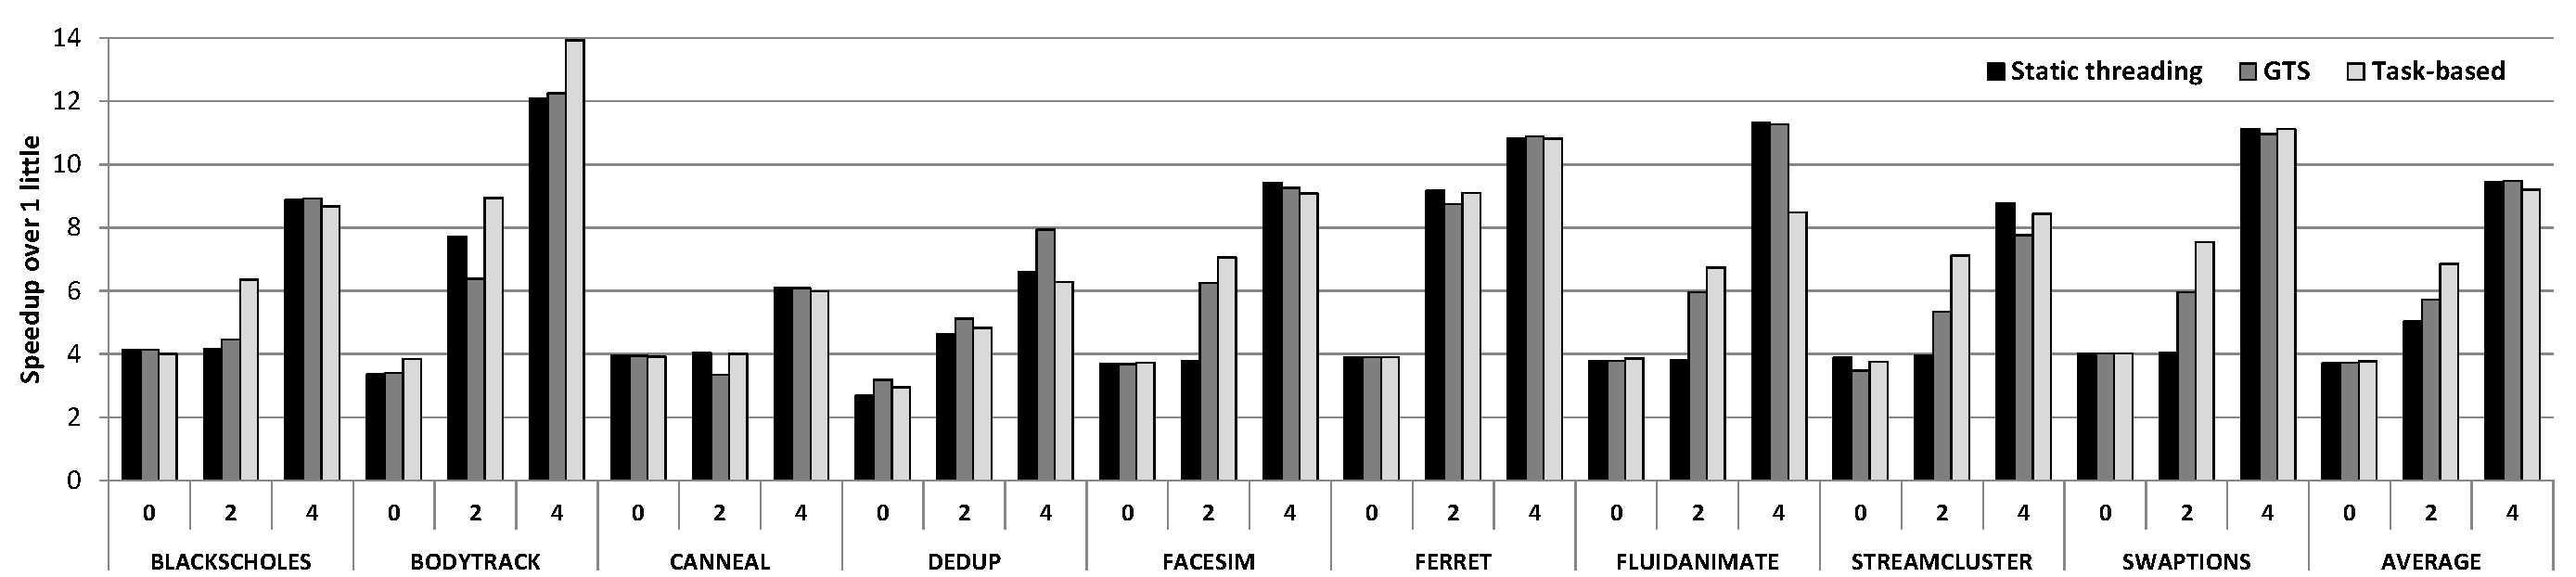
\includegraphics[width=1.0\textwidth]{figures/speedup-4.pdf}
	\vspace{-0.5cm}
	\caption{Execution time speedup over 1 little core for systems that consist of 4 cores in total with 0, 2 and 4 big cores.}
	%\caption{Performance improvements on a big.LITTLE processor with different $(F,N)$ configurations, where $F$ is the total number of big cores and $N$ the total number of cores. Results are normalized to running on four little cores with pinned Pthreads.}%
	\label{fig:speedup4}%
	\vspace{-0.3cm}
\end{figure*}

\begin{figure*}[t]%
	\centering
	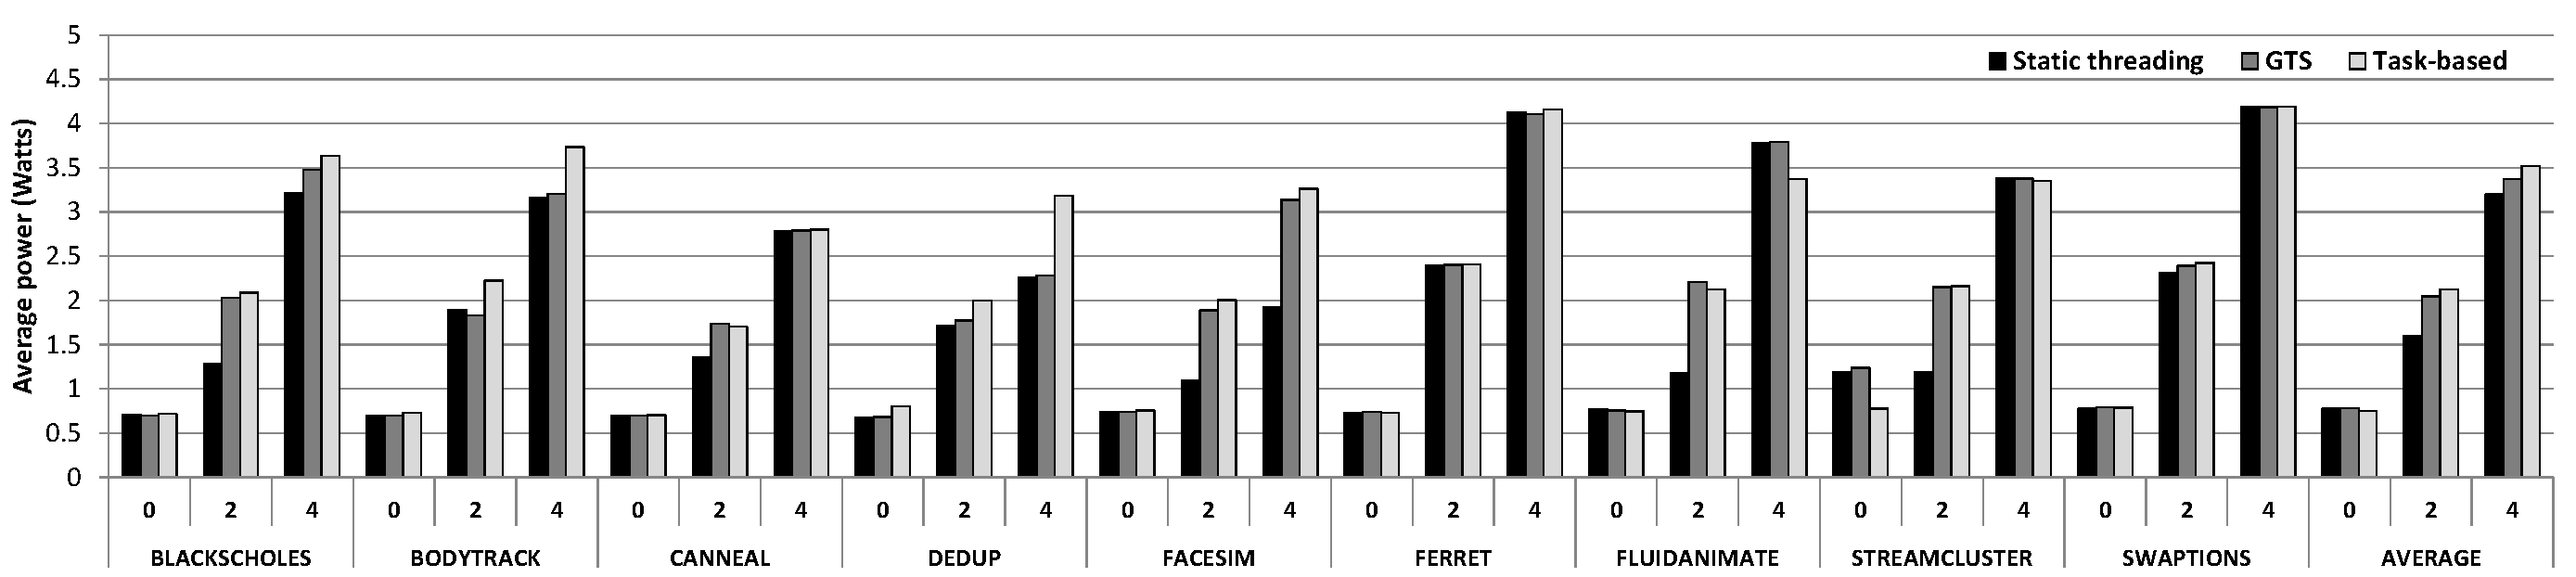
\includegraphics[width=1.0\textwidth]{figures/power4.pdf}
	\vspace{-0.5cm}
	\caption{Average power measurements on a 4-core system with 0, 2, and 4 big cores.}
	%\caption{Performance improvements on a big.LITTLE processor with different $(F,N)$ configurations, where $F$ is the total number of big cores and $N$ the total number of cores. Results are normalized to running on four little cores with pinned Pthreads.}%
	\label{fig:power4}%
	\vspace{-0.3cm}
\end{figure*}

\begin{figure*}[t]%
	\centering
	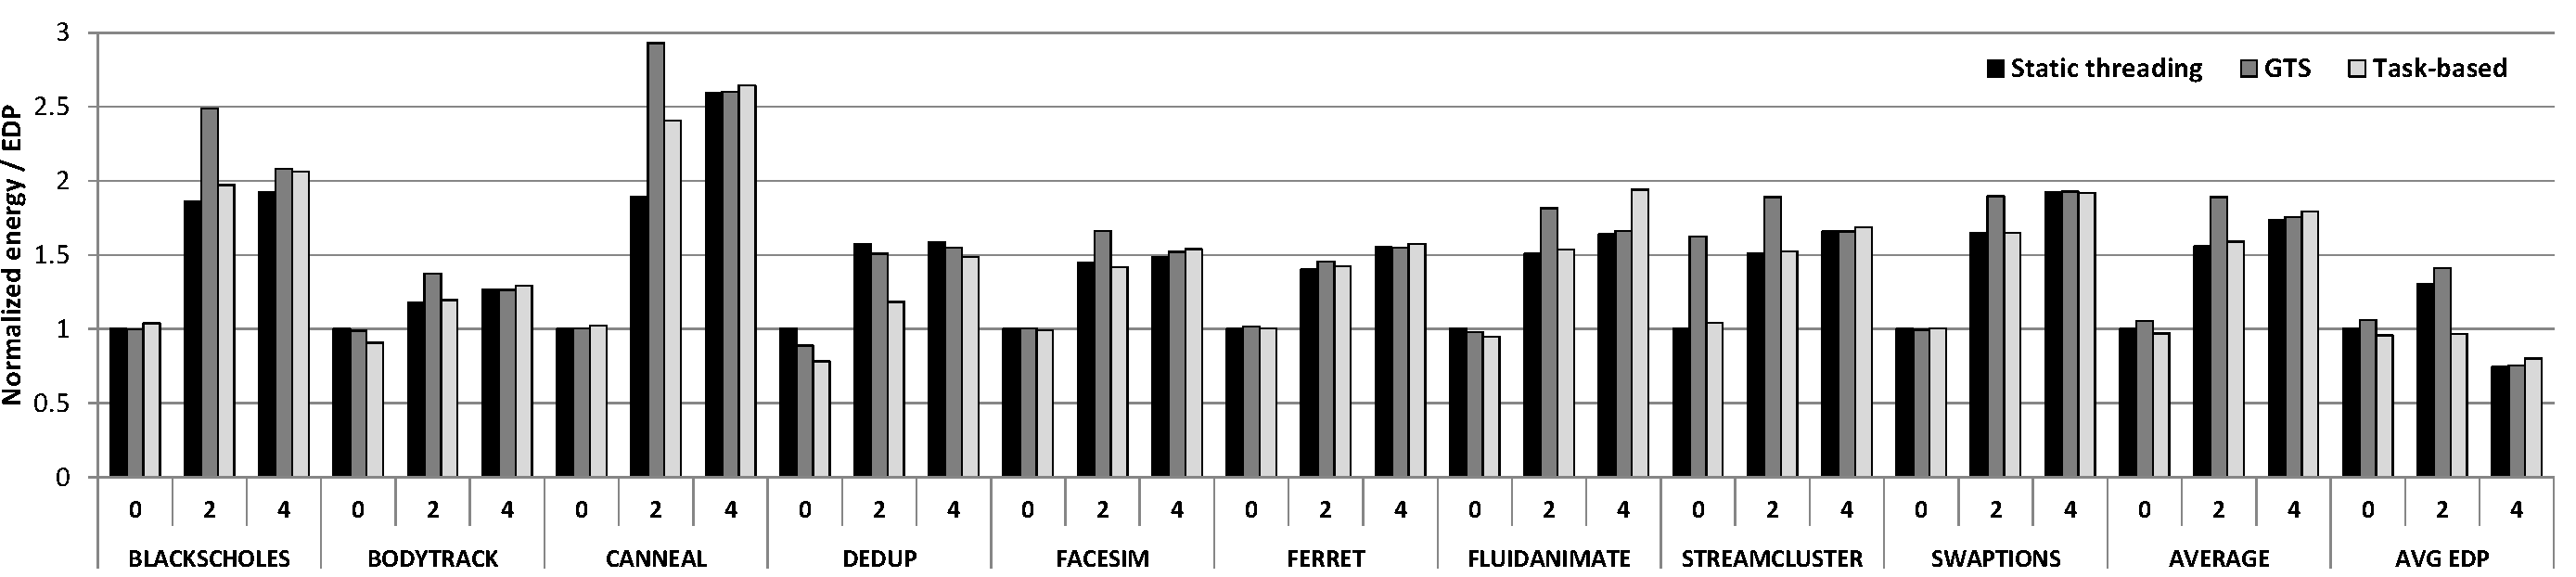
\includegraphics[width=1.0\textwidth]{figures/energy_EDP-4.pdf}
	\vspace{-0.5cm}
	\caption{Normalized energy consumption and average EDP on a 4-core system with 0, 2, and 4 big cores. Static threading with 4 little cores is used as baseline in both cases. }
	%\caption{Performance improvements on a big.LITTLE processor with different $(F,N)$ configurations, where $F$ is the total number of big cores and $N$ the total number of cores. Results are normalized to running on four little cores with pinned Pthreads.}%
	\label{fig:energy4}%
	\vspace{-0.3cm}
\end{figure*}

% \mm{We don't need to include Figure~\ref{fig:edp4} as its average results are already in the previous figure.}
% \begin{figure*}[t]%
% 	\centering
% 	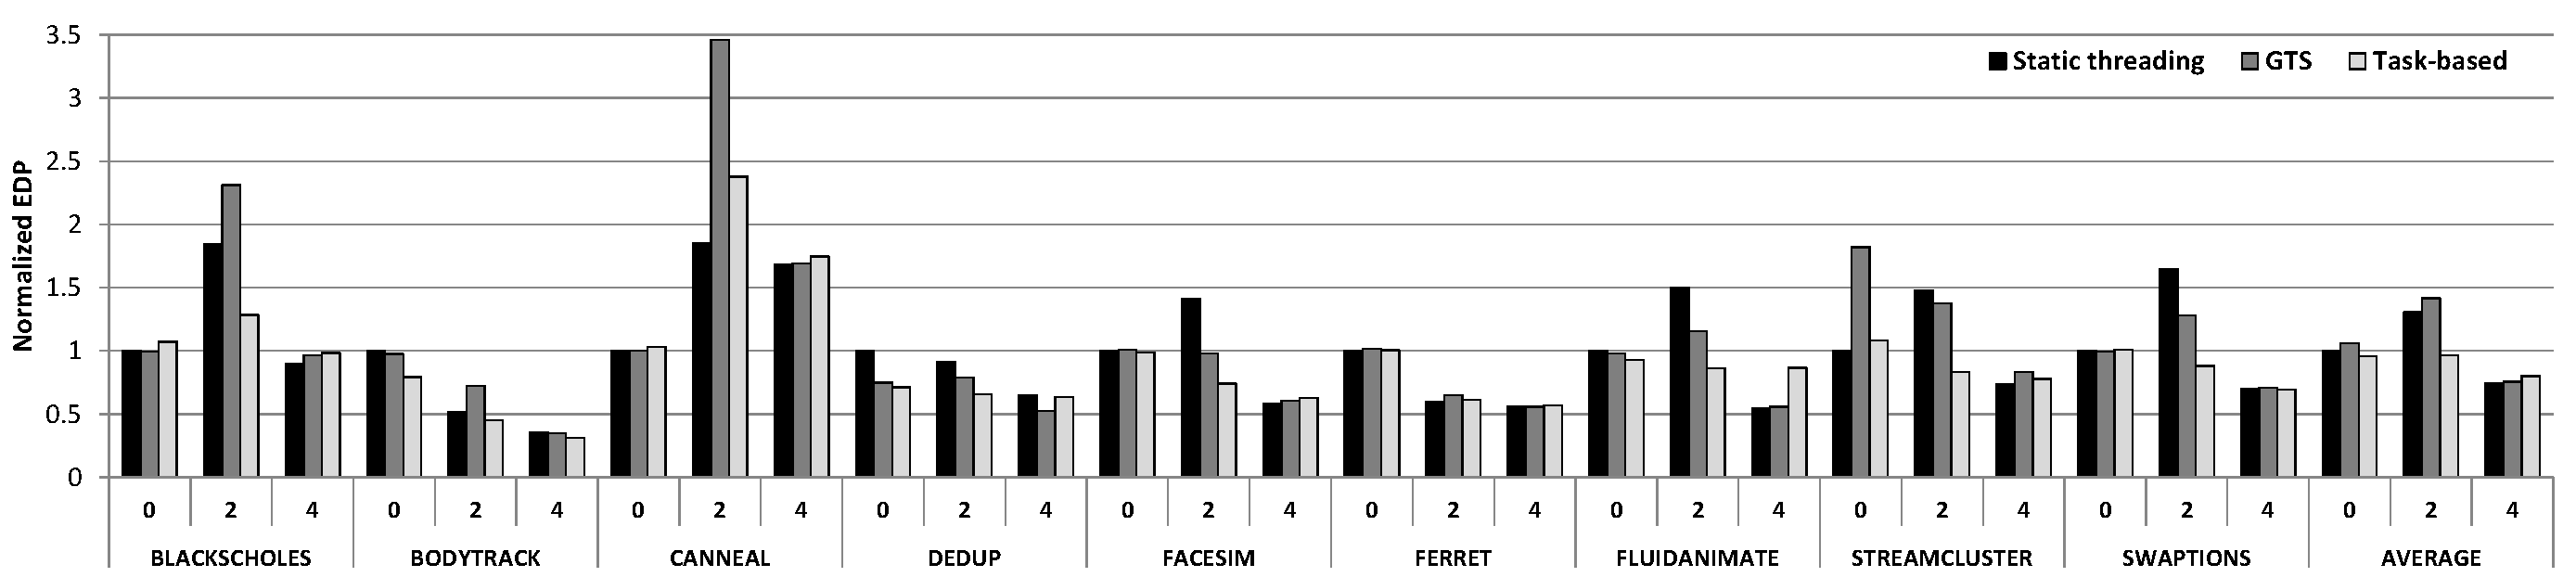
\includegraphics[width=1.0\textwidth]{figures/edp4.pdf}
% 	\vspace{-0.3cm}
% 	\caption{Normalized EDP on a 4-core system with 0, 2, and 4 big cores. Results are normalized with respect to static-threading EDP results with 4 little cores.}
% 	%\caption{Performance improvements on a big.LITTLE processor with different $(F,N)$ configurations, where $F$ is the total number of big cores and $N$ the total number of cores. Results are normalized to running on four little cores with pinned Pthreads.}%
% 	\label{fig:edp4}%
% \end{figure*}


% \begin{figure*}[t]%
% 	\centering
% 	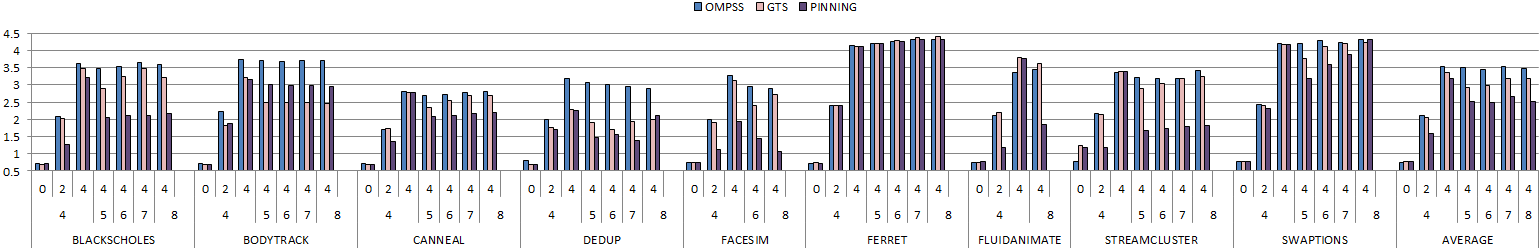
\includegraphics[width=1.0\textwidth]{figures/power-parsec}
% 	\vspace{-0.3cm}
% 	\caption{Average power consumption on a big.LITTLE processor with different $(F,N)$ configurations, where $F$ is the total number of big cores and $N$ the total number of cores.}%
% 	\label{fig:all-power}%
% \end{figure*}
% 
% \begin{figure*}[t]%
% 	\centering
% 	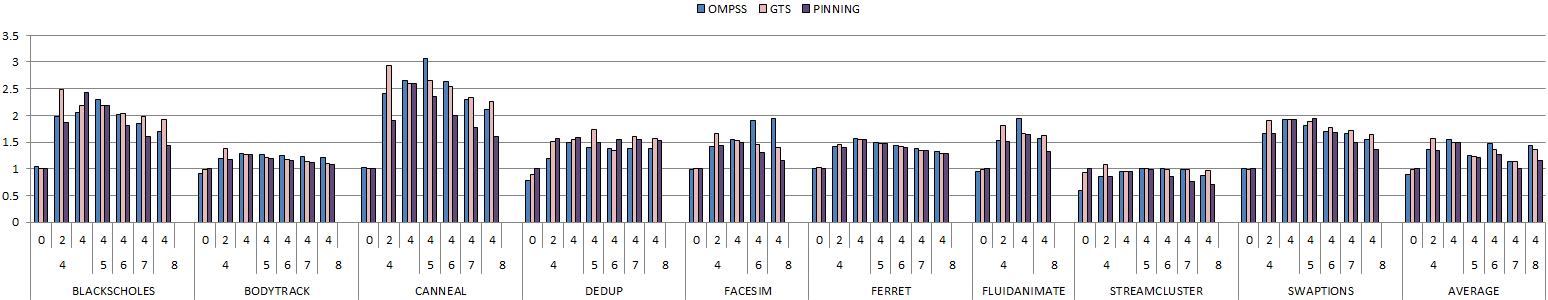
\includegraphics[width=1.0\textwidth]{figures/energy-parsec}%
% 	\vspace{-0.3cm}
% 	\caption{Energy consumption on a big.LITTLE processor with different $(F,N)$ configurations, where $F$ is the total number of big cores and $N$ the total number of cores. Results are normalized to running on four little cores with pinned Pthreads.}%
% 	\label{fig:all-energy}%
% \end{figure*}
% 
% 
% 
% \begin{figure*}[t]%
% 	\centering
% 	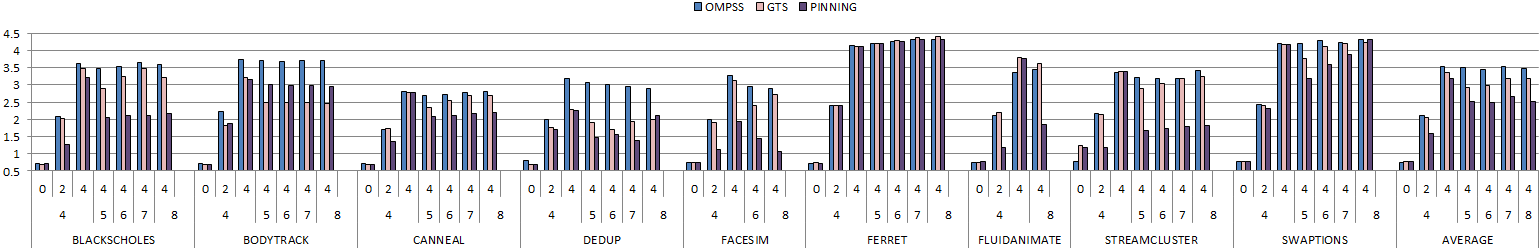
\includegraphics[width=1.0\textwidth]{figures/power-parsec}
% 	\vspace{-0.3cm}
% 	\caption{Average power consumption on a big.LITTLE processor with different $(F,N)$ configurations, where $F$ is the total number of big cores and $N$ the total number of cores.}%
% 	\label{fig:all-power}%
% \end{figure*}
% 
% \begin{figure*}[t]%
% 	\centering
% 	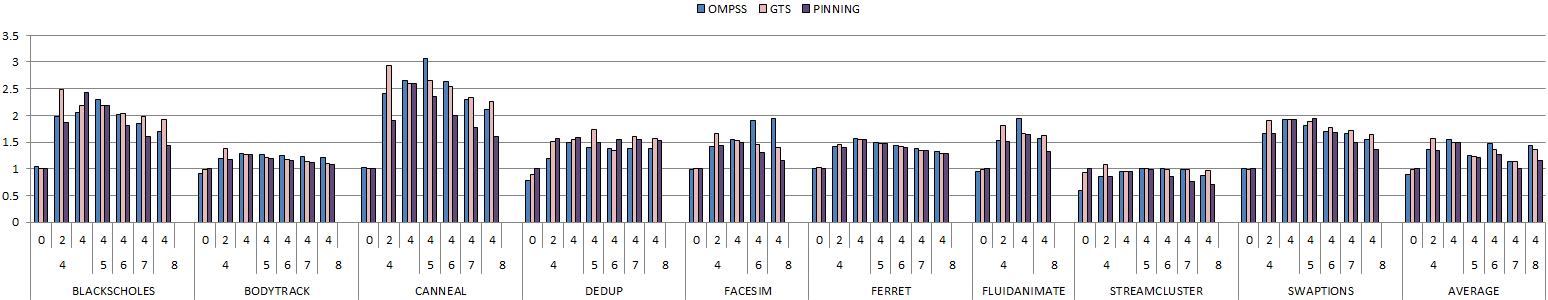
\includegraphics[width=1.0\textwidth]{figures/energy-parsec}%
% 	\vspace{-0.3cm}
% 	\caption{Energy consumption on a big.LITTLE processor with different $(F,N)$ configurations, where $F$ is the total number of big cores and $N$ the total number of cores. Results are normalized to running on four little cores with pinned Pthreads.}%
% 	\label{fig:all-energy}%
% \end{figure*}



As described in the previous section, we measure the execution time, power, energy and EDP of nine applications from the PARSEC benchmark suite~\cite{Bienia:PhD2011}. We compare these metrics  for three different scheduling approaches:
\begin{itemize}
\item \textit{Static threading}: scheduling decisions are made at the application level. The OS is not allowed to migrate threads between the clusters of big and little cores. 
\item \textit{GTS}\footnote{As this is the most advanced integrated scheduling approach supported currently, we choose to evaluate this instead of CS and IKS}: dynamic coarse-grained OS scheduling using the Global Task Scheduler integrated in the Linux kernel~\cite{samsung, ARM} using the default PARSEC benchmarks. 
\item \textit{Task-based}: dynamic fine-grained scheduling at runtime level with the task-based implementations of the benchmarks provided in PARSECSs~\cite{Chasapis:TACO2016}.
\end{itemize}


%%%%%%%%%%%%%%%%%%%%%%%%%%%%%%%%%%%%%%%%%%
%%%%%%%%%%%%%%%%%%%%%%%%%%%%%%%%%%%%%%%%%%
\subsection{Exploiting Parallelism in Asymmetric Multi-Cores}

% \mm{This section should focus on identifying the problems that current applications have on an asymmetric/heterogeneous multicore. For example, static scheduling, homogeneous domain/workload partition. More dynamic applications, will scale better (bodytrack, dedup, ferret, freqmine, vips).}

This section examines the opportunities and challenges that current asymmetric multi-cores offer to emerging parallel applications. With this objective, we first evaluate a system with a constant number of four cores, changing the level of asymmetry to evaluate the characteristics of each configuration. In these experiments, all applications run with the original parallelization strategy that relies on the user to balance the application (denoted \emph{Static threading}). The OS-based dynamic scheduling (denoted \emph{GTS}) and the task-based runtime dynamic scheduling (denoted \emph{Task-based}) are also evaluated for the same applications. 
% Figure~\ref{fig:ideal} shows the ideal speedup of the system for all the different combination of big and little cores. 
The system configurations evaluated in this section are the following:
\begin{itemize}
\item Four little cores (\texttt{0+4})
\item Two big and two little cores (\texttt{2+2})
\item Four big cores (\texttt{4+0})
\end{itemize}
For these configurations, Figure~\ref{fig:speedup4} shows the speedup of the PARSEC benchmarks with respect to running on a single little core. Figure~\ref{fig:power4} reports the average power dissipated on the evaluated platform. Finally, Figure~\ref{fig:energy4} shows the total energy consumed per application for the same configurations. Energy results are normalized to the energy measured with four little cores (higher values imply higher energy consumptions). Average EDP results are also included in this figure.

Focusing on the average performance results, we first notice that all approaches perform similarly for the homogeneous configurations. Specifically, applications obtain the best performance on the configuration with four big cores, with an average speedup of 9.5$\times$ over one little core. When using four little cores, an average speedup of 3.8$\times$ is reached for all the approaches; this shows that all the parallelization strategies are effective for this core count. In the asymmetric configuration, \emph{Static threading} slightly improves the performance (5.0$\times$ speedup), while \emph{GTS} and \emph{Task-based} reach significantly higher speedups: 5.9$\times$ and 6.8$\times$, respectively.

Contrarily, in terms of power and energy, the most efficient configuration is running with four little cores, as the performance ratio between the different cores is inversely proportional to the power ratio~\cite{Greenhalgh2011}. On average, all the approaches reach a power dissipation of 0.75W for the \texttt{0+4} configuration, while \emph{Task-based} reaches 3.5W for the \texttt{4+0} configuration, the configuration with the highest average power dissipation. It is interesting to note that in configuration \texttt{2+2}, average energy values for \emph{Static threading} and \emph{Task-based} are nearly the same, as the increase in power from 1.6W to 2.1W is compensated by a significant improvement in performance of 36\%.

Finally, in terms of EDP the best configuration corresponds to using the four big cores, as the performance improvements compensate the increase in total energy. It is worth noting that in configuration \texttt{2+2}, \emph{Task-based} achieves the same EDP results as in \texttt{0+4}, but with 55\% better performance. For the asymmetric configuration the \emph{Task-based} approach achieves the best combination of performance and energy since its dynamic scheduling is effectively utilizing the little cores. 

%\texttt{0+4} reaches a power dissipation of 0.75W with all approaches, while \emph{Task-based} reaches 3.5W in configuration \texttt{4+0}.

Thus, if the number of cores remains constant, the best configuration in terms of performance and EDP corresponds to a symmetric configuration with big cores (e.g. \texttt{4+0}), while in terms of power and energy the best configuration corresponds to a symmetric configuration with little cores (e.g. \texttt{0+4}). 
% From the average energy-delay product (EDP) results in Figure~\ref{fig:energy4} we can approximate the configuration that achieves the highest performance with the best possible energy consumption. The configuration with the lowest EDP is the one with four big cores (\texttt{4+0}) since all the scheduling approaches manage to compensate the additional energy consumption with the speedup that can be achieved on this set-up. However, it is interesting to note that for the asymmetric configuration the \emph{Task-based} approach achieves the best combination of performance and energy since its dynamic scheduling approach is effectively utilizing the little cores. 

\begin{figure*}[t]%
	\centering
	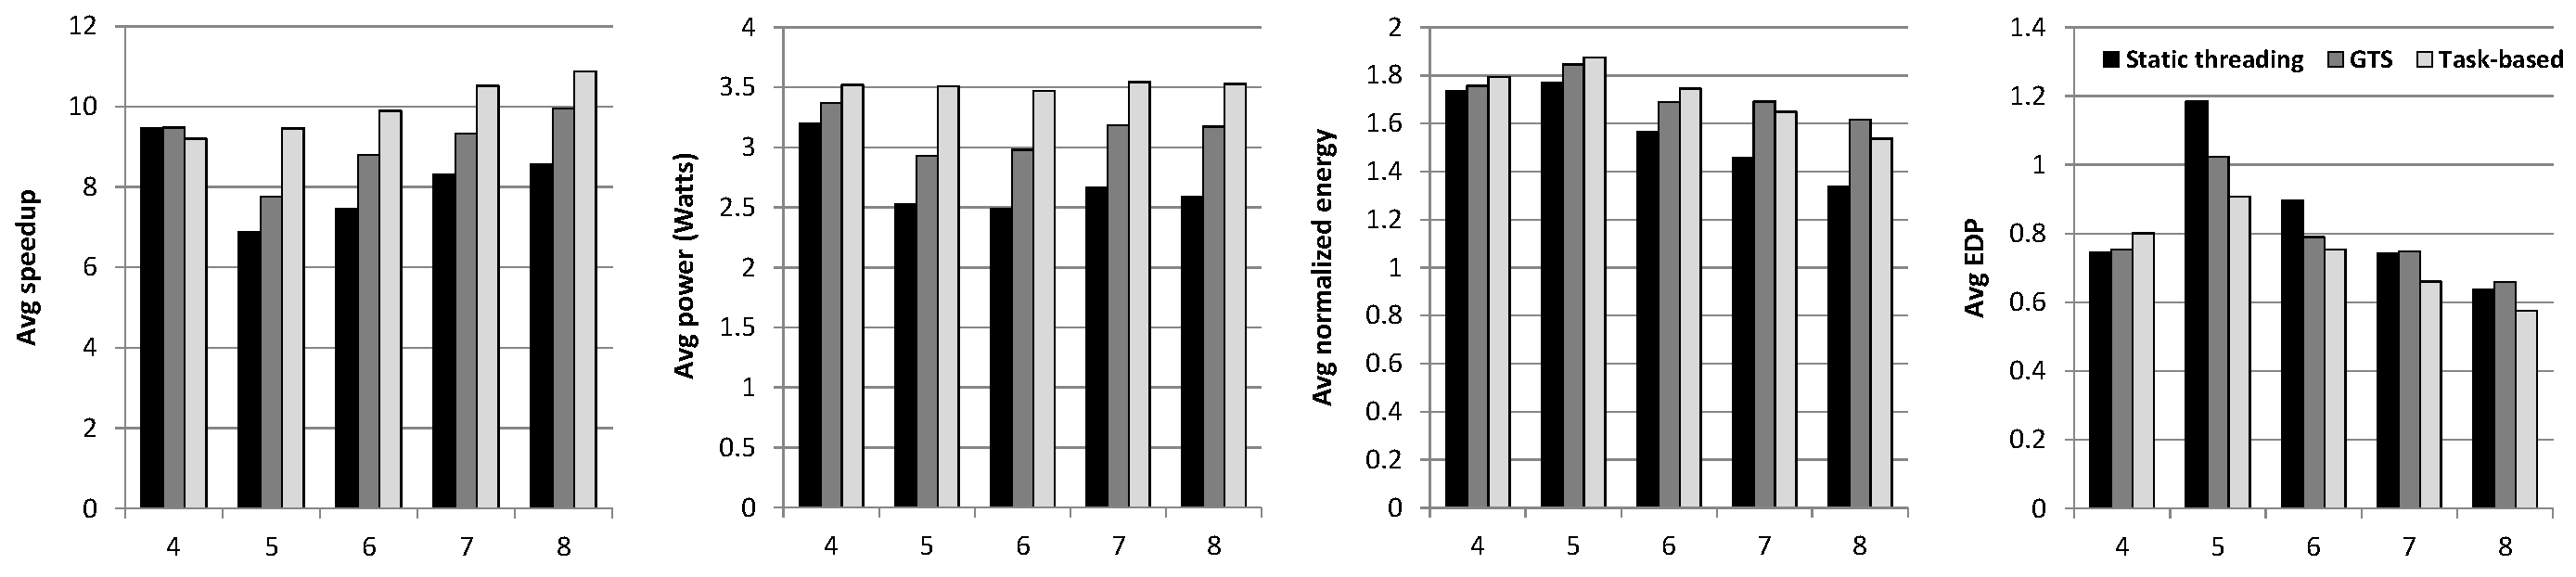
\includegraphics[width=\textwidth]{figures/averages_4plus.pdf}
	\vspace{-0.5cm}
	\caption{Average results when running on 4 to  8 cores with 4 of them big. Speedup is over 1 little core, static threading on 4 little cores is the baseline of energy consumption and EDP}
	%\caption{Performance improvements on a big.LITTLE processor with different $(F,N)$ configurations, where $F$ is the total number of big cores and $N$ the total number of cores. Results are normalized to running on four little cores with pinned Pthreads.}%
	\label{fig:averages4plus}%
	\vspace{-0.3cm}
\end{figure*}


Next, we focus on the obtained results per benchmark. For applications with an extensive use of barriers (blackscholes, facesim, fluidanimate, streamcluster and swaptions) or with a memory intensive pattern (canneal), the extra computational power offered by the big cores in configuration \texttt{2+2} is not exploited. As a result with \emph{Static threading} performance is only slightly improved by 1\% on average when moving from \texttt{0+4} to the \texttt{2+2} configuration. This slight improvement comes at the cost of much more power and energy consumption (79\% and 64\% respectively).
%As a result, with \emph{Static threading} the performance equals the one of the configuration \texttt{0+4} (average 1\% improvement), but at the expense of much more power and energy consumption (79\% and 64\% increase, respectively). 
These results are explained three-fold: i) load is distributed homogeneously among threads in some applications; ii) extensive usage of barriers force big cores to wait until little cores reach the barrier; and iii) high miss rates in the last-level cache cause frequent pipeline stalls and prevent to fully exploit the computational power of big cores. To alleviate these problems, the programmer should develop more advanced parallelization strategies that could benefit from asymmetric cores, as performed in the remaining applications, or rely on a dynamic scheduling approach at OS or runtime levels.

The three remaining applications are parallelized using a pipeline model (bodytrack, dedup, and ferret)  with queues for the data-exchange between pipeline stages and application-specific load balancing mechanisms designed by the programmer. As a result, \emph{Static scheduling} with these applications benefits from the extra computational power of the big cores in the configuration \texttt{2+2}. These mechanisms are not needed in the \emph{Task-based} code; in this approach the code of the application is simplified and the runtime automatically allows the overlapping of the different pipeline stages. As a result, \emph{Task-based} further improves the obtained performance, reaching a 13\% average improvement over \emph{GTS}. It is clear that these applications benefit in performance by the increased number of big cores, while power and energy are increasing since the big cores are effectively utilized.

%In these applications, all the approaches clearly outperform configuration \texttt{0+4}, while still increasing power and energy, as now all cores are busy (not only the little ones).

%the parallel regions to overlap more aggressively different stages of the pipeline. As a result, \emph{Task-based} further improves the obtained performance, reaching a 13\% average speedup over \emph{GTS}. In these applications, all the approaches clearly outperform configuration \texttt{0+4}, while still increasing power and energy, as now all cores are busy (not only the little ones).

Generally, relying on the programmer to benefit from asymmetry does not report good results, as it is very hard to predict the system's behaviour on application-level. Only when applications implement advanced features with user-level schedulers and load balancing techniques, they can benefit from asymmetry, of course at the cost of programmability effort. Relying on the OS is a suitable alternative but the optimal one is relying on the runtime to dynamically schedule tasks on the asymmetric processor, reaching much better performance, power and energy results.

%the developer did not consider it when designing the parallelization technique. When applications implement advanced features with user-level schedulers and load balancing techniques, applications can benefit from asymmetry, of course at the cost of programmability effort. A suitable alternative consists in relying on the OS system or the runtime to dynamically schedule tasks into the asymmetric processor, reaching much better performance, power and energy results in these systems.


%To estimate the best configuration when taking into account both performance and energy efficiency we have to 


%Relying on the programmer to benefit from asymmetry does not report good results, as the developer did not consider it when designing the parallelization technique. When applications implement advanced features with user-level schedulers and load balancing techniques, applications can benefit from asymmetry, of course at the cost of programmability effort. A suitable alternative consists in relying on the OS system or the runtime to dynamically schedule tasks into the asymmetric processor, reaching much better performance, power and energy results in these systems.

%, power or energy corresponds to a homogeneous configuration with in-order cores (power and energy) or big cores (performance). 

%In general relying on the programmer to benefit from asymmetry does not report good results, as the developer did not consider it when designing the parallelization technique. When applications implement advanced features with user-level schedulers and load balancing techniques, applications can benefit from asymmetry, of course at the cost of programmability effort. A suitable alternative consists in relying on the OS system or the runtime to dynamically schedule tasks into the asymmetric processor, reaching much better performance, power and energy results in these systems.
\iffalse
\mm{Figure~\ref{fig:energy4} also shows the average normalized results for EDP. In this case, lower is better. I didn't comment these results yet. With this metric, Task-based on 2+2 is as good as the others in 0+4 while we obtain better performance. This is interesting, but I'm not sure if it adds much with respect to the already presented numbers.}

\mm{I haven't commented much the results with the GTS scheduler. Maybe we should extend this part. Next, I put some sentences that might be useful, although I don't know where to put them.}

As described in Section~\ref{sec:scheduling}, the Global Task Scheduler (GTS) migrates tasks between cores in order to balance the load in the different cores of the heterogeneous processor. 

For fork-join + homogeneous load, the scheduler should be very effective, reaching the performance results of OmpSs. However, it is unaware of what it is moving around, which means that it might move a thread that is idle to a big core...

Consequently, for some benchmarks, the OS is making decisions without coordinating with the application scheduler and can worsen the performance. This should be the case of the applications with advanced load balancing techniques, but I still don't know if we will see this behavior.
\fi
\begin{figure*}[t]%
	\centering
	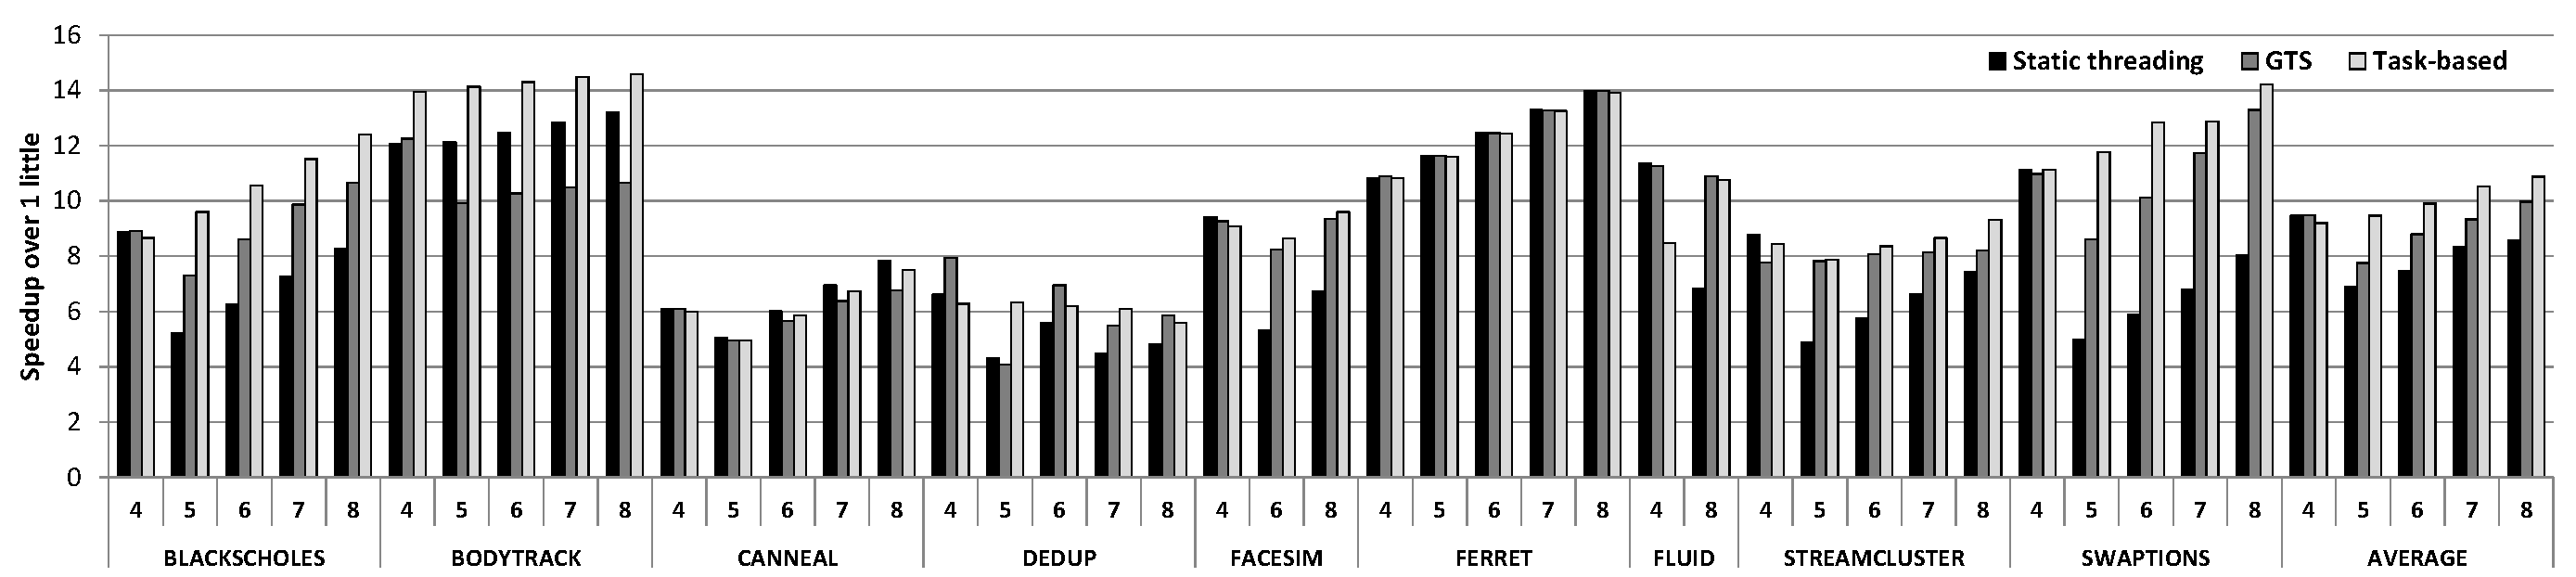
\includegraphics[width=1.0\textwidth]{figures/speedup-4plus.pdf}
	\vspace{-0.5cm}
	\caption{Speedup over 1 little core when running on 4 to 8 cores and 4 of them are big}
	%\caption{Performance improvements on a big.LITTLE processor with different $(F,N)$ configurations, where $F$ is the total number of big cores and $N$ the total number of cores. Results are normalized to running on four little cores with pinned Pthreads.}%
	\label{fig:speedup4plus}%
	\vspace{-0.3cm}
\end{figure*}

\begin{figure*}[t]%
	\centering
	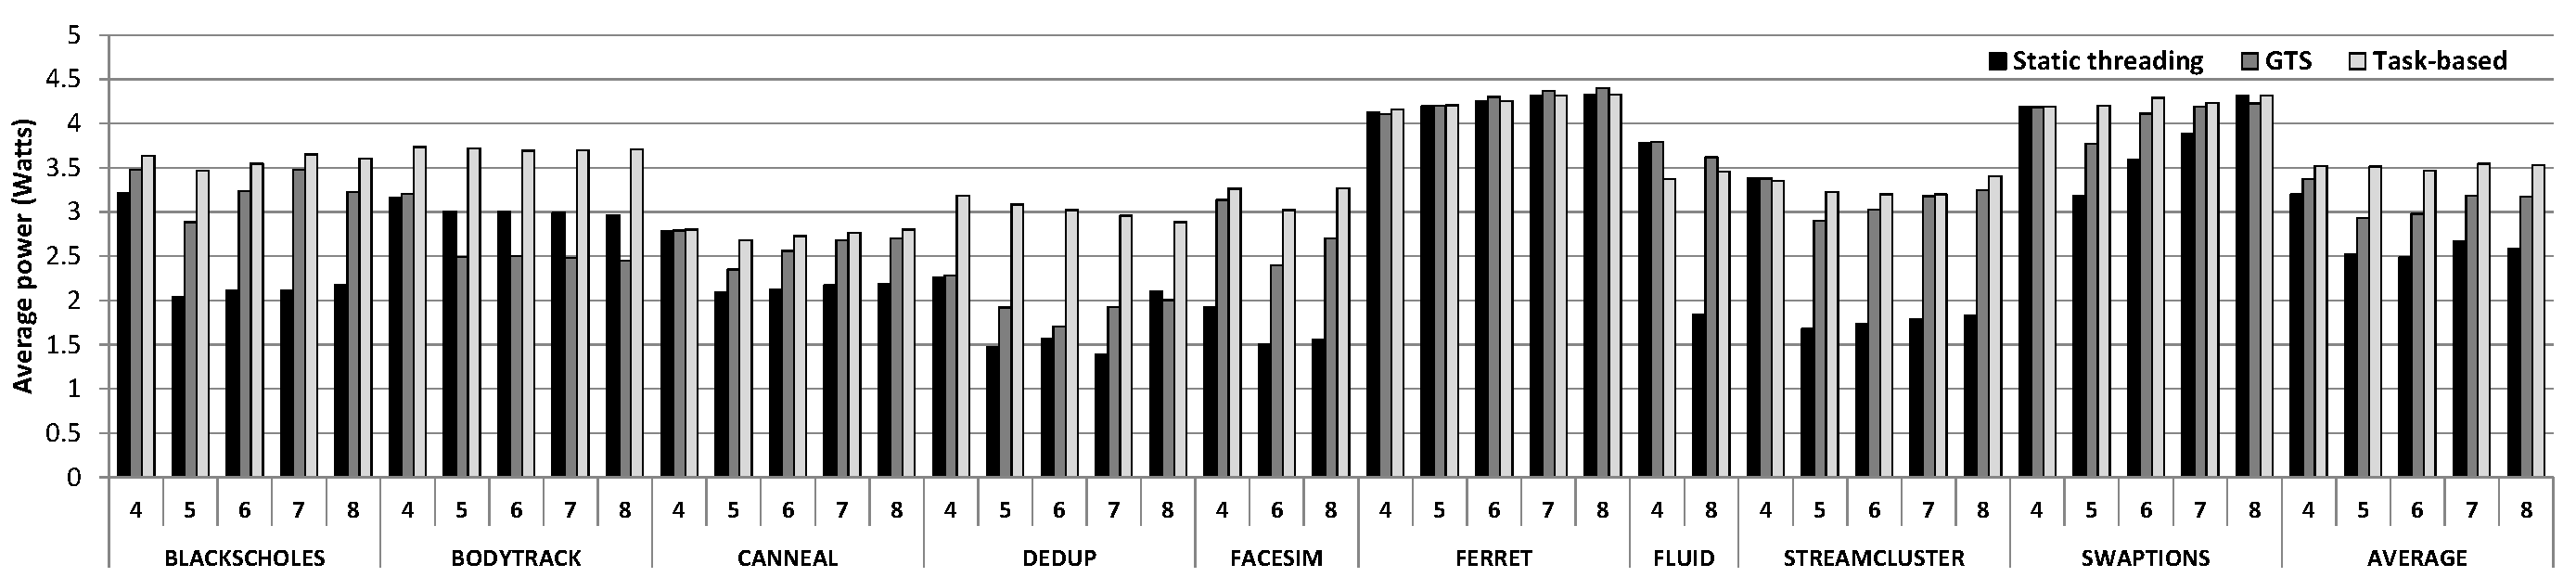
\includegraphics[width=1.0\textwidth]{figures/power4plus.pdf}
	\vspace{-0.5cm}
	\caption{Average power when running on 4 to 8 cores and 4 of them are big}
	%\caption{Performance improvements on a big.LITTLE processor with different $(F,N)$ configurations, where $F$ is the total number of big cores and $N$ the total number of cores. Results are normalized to running on four little cores with pinned Pthreads.}%
	\label{fig:power4plus}%
	\vspace{-0.3cm}
\end{figure*}

% \begin{figure*}[t]%
% 	\centering
% 	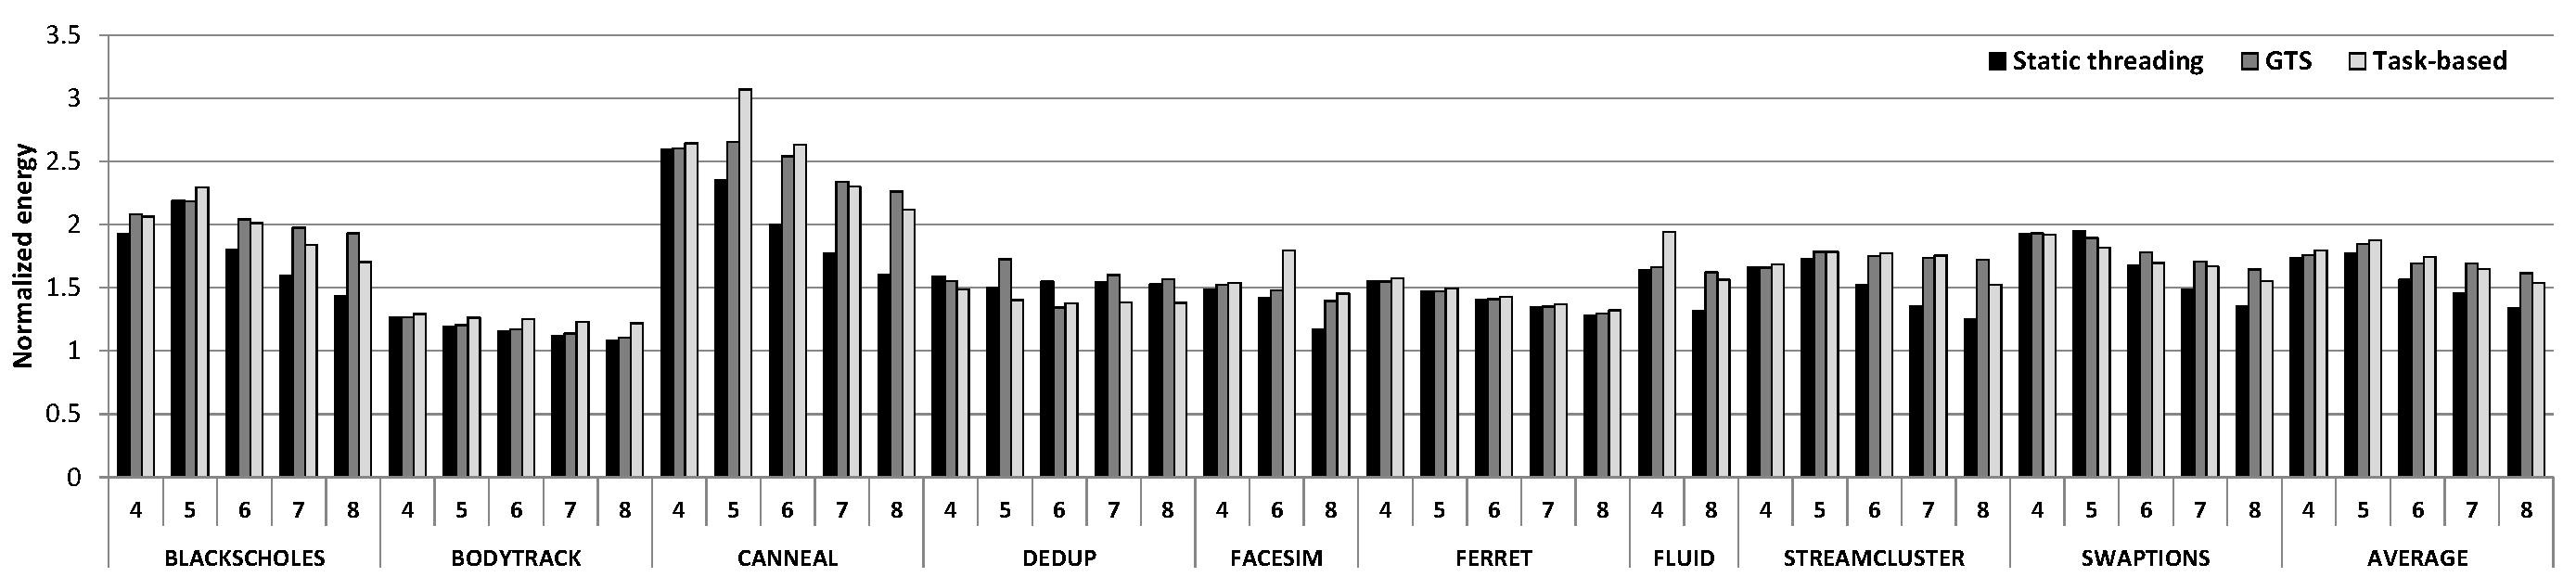
\includegraphics[width=1.0\textwidth]{figures/energy-4plus.pdf}
% 	\vspace{-0.5cm}
% 	\caption{Normalized energy consumption with respect to 4-little-static-threading energy consumption, when running on 4 to 8 cores and 4 of them are big}
% 	%\caption{Performance improvements on a big.LITTLE processor with different $(F,N)$ configurations, where $F$ is the total number of big cores and $N$ the total number of cores. Results are normalized to running on four little cores with pinned Pthreads.}%
% 	\label{fig:energy4plus}%
% 	\vspace{-0.3cm}
% \end{figure*}

% \begin{figure*}[t]%
% 	\centering
% 	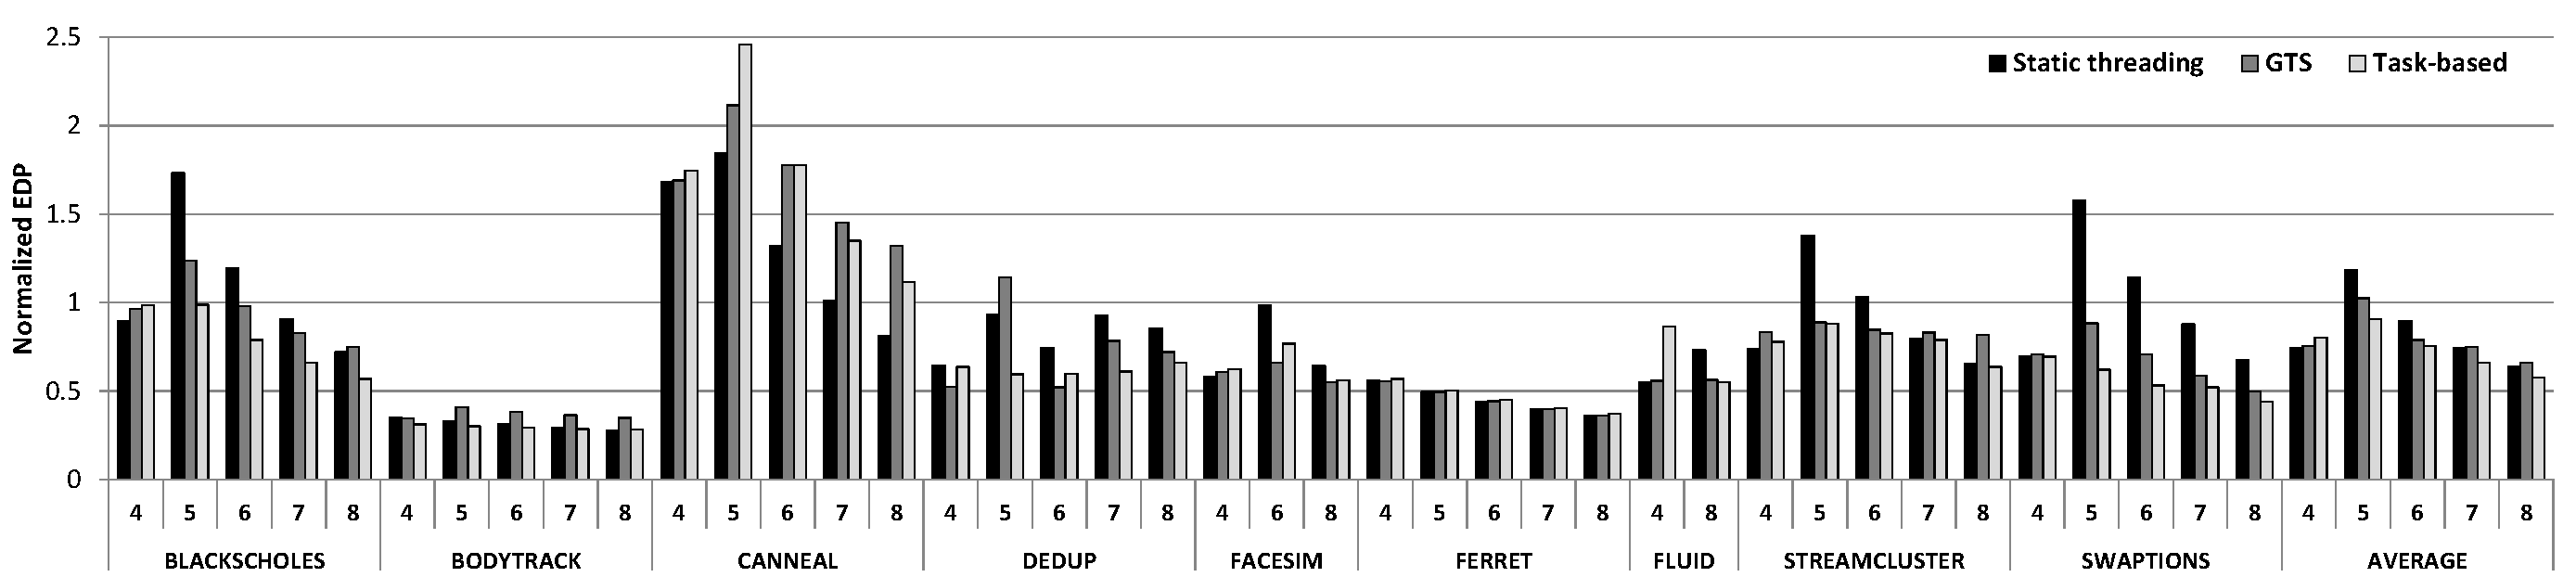
\includegraphics[width=1.0\textwidth]{figures/edp4plus.pdf}
% 	\vspace{-0.3cm}
% 	\caption{Normalized EDP when running on 5, 6, 7, or 8 cores and 4 of them are big}
% 	%\caption{Performance improvements on a big.LITTLE processor with different $(F,N)$ configurations, where $F$ is the total number of big cores and $N$ the total number of cores. Results are normalized to running on four little cores with pinned Pthreads.}%
% 	\label{fig:edp4plus}%
% \end{figure*}


%%%%%%%%%%%%%%%%%%%%%%%%%%%%%%%%%%%%%%%%%%
%%%%%%%%%%%%%%%%%%%%%%%%%%%%%%%%%%%%%%%%%%
\subsection{Adding Little Cores to a Symmetric Multi-core}

In the following experiments, we explore if an application running on a symmetric multi-core with big cores can benefit from adding small cores that help in its execution. Having more computational resources increases the ideal speedup a parallel application can reach, but it also introduces challenges at application, runtime and OS level. Thus, we want to see how many small cores have to be added to the system to compensate the cons of having to deal with asymmetry in the evaluated approaches.

To evaluate this scenario, we explore configurations \texttt{4+0}, \texttt{4+1}, \texttt{4+2}, \texttt{4+3} and \texttt{4+4}. In these experiments, the number of big cores remains constant (four), while the number of little cores increases from 0 to 4. First we focus on the average results of speedup, power, energy and EDP, shown in Figure~\ref{fig:averages4plus}.

The speedup chart of Figure~\ref{fig:averages4plus} shows that the \emph{Static threading} approach does not benefit from adding little cores to the system.
In fact, this approach brings an average 15\% slowdown when adding four little cores for execution (configuration \texttt{4+4}).
This is a result of the static thread scheduling; because the same amount of work is assigned to each core, when the big cores finish the execution of their part, they will become idle and under-utilized. 
GTS achieves a limited speedup of 5\% with the addition of four little cores to the \texttt{4+0} configuration. The addition of a single little core brings a 22\% slowdown (from \texttt{4+0} to \texttt{4+1}) and requires three additional little cores to match the performance of the symmetric configuration (configuration \texttt{4+3}).  Finally, the \emph{Task-based} approach always benefits from the extra computational power as the runtime automatically deals with load imbalance. Performance improvements keep growing with the additional little cores, reaching an average improvement of 16\% over the symmetric configuration when 4 extra cores are added. An interesting observation is that according to the ideal speedup (Equation~\ref{eq.ideal} and Figure~\ref{fig:ideal}), the average ideal performance increase when moving from the \texttt{4+0} configuration to the \texttt{4+4} is 33\%, considering that the average performance ratio is 2.96$\times$ as shown in Table~\ref{tab:parsec}. Thus, the task-based approach achieves almost half of this theoretical ideal performance.

%the execution time speedup of the PARSEC benchmarks with respect to running in a single in-order core. 
%When looking at the average results, it is very interesting to see that the \emph{Static threading} approach clearly fails to benefit from the extra in-order cores. Even with four extra cores (configuration \texttt{4+4}), an average 15\% slowdown is obtained. \emph{GTS} also suffers a significant performance reduction when adding an extra little core (22\% slowdown) and requires three additional little cores to match the performance of the symmetric configuration. With an additional extra core, \emph{GTS} reaches an average 5\% speedup over the symmetric configuration. 



%In contrast, the \emph{Task-based} approach always benefits from the extra computational power as the runtime automatically deals with load imbalance. Performance improvements keep growing with the additional little cores, reaching an average improvement of 16\% over the symmetric configuration when 4 extra cores are added. Please, note that according to Table~\ref{tab:parsec} the performance ratio between big and little cores is 2.96$\times$, which means that the ideal speedup when adding 4 little cores to a system with 4 big cores is 1.33$\times$ ($\frac{2.96\cdot 4 + 4}{2.96\cdot 4}$). Thus, the \emph{Task-based} approach reaches half of the potential speedup on this asymmetric platform.

The power chart of Figure~\ref{fig:averages4plus} shows oppositional benefits among the three approaches. We can see that \emph{Static threading} and \emph{GTS} benefit from asymmetry, effectively reducing average power consumption.
\emph{Static threading} reduces power consumption when moving from the \texttt{4+0} to the \texttt{4+4} system by 23\% while \emph{GTS} does so by 6.2\%.
On the other hand, the \emph{task-based} approach keeps the big cores busy for most of the time so it maintains the average power nearly constant.



%In terms of power, the tradeoffs completely change. As shown in Figure~\ref{fig:power4plus}, \emph{Static threading} and \emph{GTS} always benefit from asymmetry, effectively reducing average power consumption. On average in configuration \texttt{4+4}, \emph{Static threading} and \emph{GTS} reduce power 23\% and 6.2\%, respectively, with respect to the symmetric multi-core. In contrast, the \emph{Task-based} approach always has all big cores busy and maintains overall power nearly constant. 

%In terms of energy, the third chart of Figure~\ref{fig:averages4plus} shows that the \emph{Static threading} significantly reduces energy consumption by 31\% when moving from \texttt{4+0} to the \texttt{4+4} configuration. As shown in the previous section, little cores are more energy efficient than big cores, at the cost of reduced performance. In the case of \emph{GTS} and \emph{Task-based}, at least two extra cores are needed to reduce energy. 
% In configuration \texttt{4+4}, energy is reduced by 31\% for \emph{Static threading}, 9.3\% for \emph{GTS}, and 16\% for \emph{Task-based}. Consequently, we can state that asymmetry reduces overall energy consumption, although the best configuration in terms of energy consists in using only four little cores.
\begin{figure*}
        \centering
        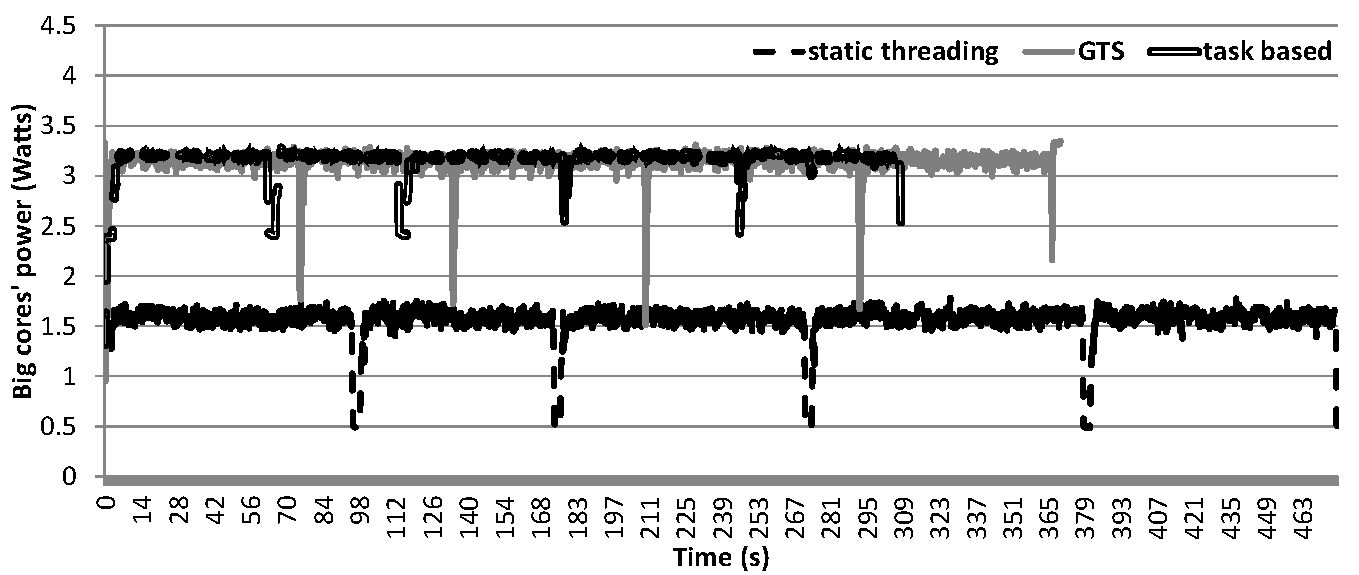
\includegraphics[width=\columnwidth]{figures/stream_samples_A15} \hspace{0.2cm}
        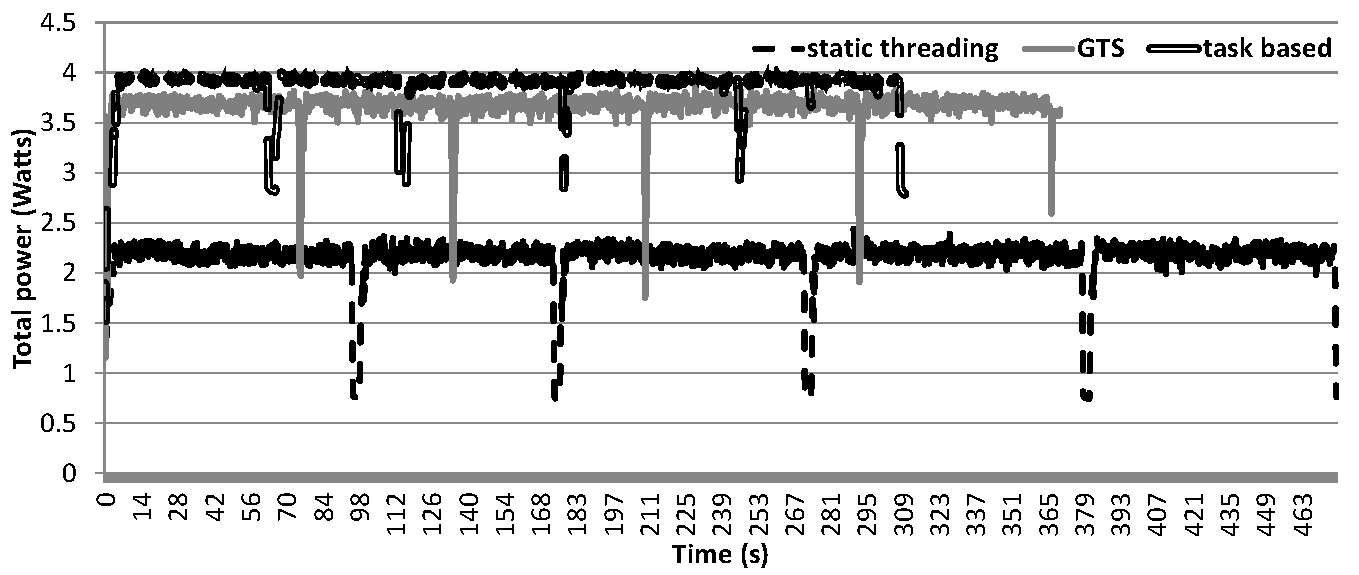
\includegraphics[width=\columnwidth]{figures/stream_samples_total}%
        \vspace{-0.3cm}
        \caption{Power consumption of the Streamcluster benchmark on the 8-core Octodroid Platform. Left: Consumption of the 4 big cores. Right: Consumption of the whole chip.}%
        \label{fig:streamcluster_consumption_evolution}%
\end{figure*}

As a result of the reduction in power, average energy results are significantly reduced in the case of \emph{Static threading} as shown on the energy chart of Figure~\ref{fig:averages4plus}. As discussed in the previous section, little cores are more energy efficient than big cores, at the cost of reduced performance. In the case of \emph{GTS} and \emph{Task-based}, at least two extra cores are needed to reduce energy. In configuration \texttt{4+4}, energy is reduced by 31\% for \emph{Static threading}, 9.3\% for \emph{GTS}, and 16\% for \emph{Task-based}. Consequently, we can state that asymmetry reduces overall energy consumption, although the best configuration in terms of energy consists in using only four little cores as average normalized energy is always above 1.

%--- ADD EDP results comments on average EDP
To see the impact on both performance and energy efficiency we plot the average energy delay product (EDP) on the rightmost chart of Figure~\ref{fig:averages4plus}. In this chart the lower values are the better. We observe that the \emph{task-based} approach is the one that has the best performance-energy combination for the asymmetric configurations since it maintains the lowest EDP for all cases. \emph{Static threading} manages to reduce the average EDP by 7\% while \emph{GTS} and \emph{task based} approaches do so by 10\% and 37\% respectively.
%---

Figure~\ref{fig:speedup4plus} shows a more detailed exploration of the performance results. According to Table~\ref{tab:parsec} the applications with barrier synchronization are blackscholes, facesim, fluidanimate, streamcluster and swaptions. For these applications the most efficient system configuration with the \emph{Static threading} approach is the \texttt{4+0}. Little cores increase execution time due to load imbalance effects. Since the big cores reach barriers earlier, power is reduced for these applications, as shown in Figure~\ref{fig:power4plus}. Energy reduction is less significant with a few extra little cores as the performance degradation is too high, but as the number of little cores increases, energy is reduced. Moreover, the applications with more advanced load balancing techniques like pipelined parallelism are bodytrack, dedup and ferret. These applications take advantage of the asymmetric hardware and balance the load in all the cores. As a result, performance improves while we increase the number of little cores. In the case of bodytrack, \emph{GTS} reduces performance by 20\% when adding four little cores. We attribute this to the cost of the thread migration from one core to the other in contrast to the \emph{Static threading} approach that does not add such overheads. 
%\kc{Please check this and let me know if makes sense. I had to write a comment for bodytrack.} 
In the case of dedup, results show more variability. This benchmark is very I/O intensive and, depending on the type of core that executes these I/O operations, performance drastically changes. In oder to deal with this problem, a smarter dynamic scheduling mechanism would be required. Finally, canneal application does not 
scale according to its ideal speedup reported on Figure~\ref{fig:ideal} as it has a memory intensive pattern which limits performance.

Figure~\ref{fig:power4plus} shows the average power measured in each case. The barrier-synchronized applications (blackscholes, facesim, fluidanimate, streamcluster and swaptions) reduce power because of their imbalance; since big cores have long idle times with the \emph{Static threading} approach, they don't spend the same power as \emph{GTS} and \emph{Task-based}.
%the big cores reach barriers earlier and remain idle, so power is reduced for the \emph{Static threading} approach compared to \emph{GTS} and \emph{Task-based}. 
Each one of the pipeline-parallel applications bodytrack and ferret maintains nearly the same power levels among the configurations for each scheduling approach. Dedup is an exception, as the results highly depend on the core that executes the I/O operations mentioned above. However, the effect of the lower power for \emph{Static threading} is observed in all the benchmarks and is because of the big cores' long idle times.

%Each one of the pipeline-parallel applications (bodytrack, dedup, ferret) maintains nearly the same power levels among the configurations for each scheduling approach. 

%In these cases, the big cores do not remain as  Canneal also spends constant power among system configurations for the same reason.

%, while power consumption remains approximately the same. Consequently, total energy is reduced benefits in these asymmetric configurations.

%When focusing on the individual results per benchmark, the best configuration in terms of performance for applications with barriers (blackscholes, facesim, fluidanimate, streamcluster and swaptions) and with a memory intensive pattern (canneal) is \texttt{4+0}. Simple in-order cores increase execution time due to load imbalance effects. Since the big cores reach barriers earlier, power is reduced as a result for these applications, as shown in Figure~\ref{fig:power4plus}. Energy reduction is less significant with few extra little cores as the performance degradation is too high, but as the number of little cores increases, energy is reduced. 



%For applications with advanced load balancing techniques (bodytrack, dedup, and ferret), the application can take advantage of the asymmetric hardware and schedule load in all the cores. As a result, performance improves while we increase the number of little cores, while power consumption remains approximately the same. Consequently, total energy is reduced benefits in these asymmetric configurations. In the case of bodytrack, \emph{GTS} is having problems and a 20\% reduction in performance is obtained. \mm{Any idea why?}. In the case of dedup, results show more variability. This benchmark is very I/O intensive and, depending on which core executes these I/O operations, performance drastically changes. In oder to deal with this problem, a smarter dynamic scheduling mechanism would be required.

As we have seen in this section, adding little cores to a symmetric multi-core with big cores presents significant challenges for the application, OS and runtime developers. Little cores increase load imbalance and can degrade performance as a result. Relying on the application developer to deal with this asymmetry is complex and many applications are not ready. A dynamic OS scheduler such as \emph{GTS} can help in mitigating these problems, but the best results in terms of performance are obtained with the \emph{Task-based} approach. In terms of power and energy, the asymmetric multi-core provides significant benefits, although the symmetric multi-core with little cores remains the most energy-efficient configuration. The answer to the question which is the best system configuration for the higest performance the lowest energy consumption can be found on the average EDP chart of Figures~\ref{fig:energy4} and \ref{fig:averages4plus}, and is the use of the entire 8-core system with the \emph{Task based} approach.


%%%%%%%%%%%%%%%%%%%%%%%%%%%%%%%%%%%%%%%%%%
%%%%%%%%%%%%%%%%%%%%%%%%%%%%%%%%%%%%%%%%%%
\subsection{Power Consumption Analysis over Time}

%To understand in detail some of the behaviours pointed out in the last sections, we provide detailed power measurements during the whole execution of the streamcluster benchmark. 

This section provides a detailed analysis of the power consumption over time for one of the evaluated applications, streamcluster.
We choose this application because the power samples are stable and can be plotted with visibility.
Figure \ref{fig:streamcluster_consumption_evolution} shows the power samples measured over the execution time of streamcluster when running on 8 cores (\texttt{4+4} configuration).
On the left part of the figure we plot the power samples of only the 4 big cores, while on the right part we plot the total power samples of all the big and the little cores.
Both charts contain this information for the three scheduling approaches evaluated in this paper (\emph{Static threading}, \emph{GTS} and \emph{Task-based}).
As expected, all the approaches display the same five execution phases throughout the execution, as this benchmark is processing five large chunks of points.
Seemingly the power samples of the big-core cluster slightly outreach 3W for the \emph{GTS} and \emph{Task-based} approaches, while for \emph{Static threading} they remain close to 1.5W. As shown in Figure~\ref{fig:power4}, steamcluster dissipates 1.2W when running on 4 little cores.
Thus, this proves that the \emph{GTS} and \emph{Task-based} approaches better utilize the big cores and, in contrast, the big cores remain idle for a significant amount of time with the \emph{Static threading} strategy.

On the right of Figure~\ref{fig:streamcluster_consumption_evolution}, where the power samples of the whole chip are plotted, the \emph{Task-based} approach has power samples slightly higher than the \emph{GTS} approach:
with the \emph{Task-based} approach, measured power is around 4.0W, while with \emph{GTS} observed power is around 3.6W.
The main difference between these measurements and the ones on the left chart of the same figure is the power consumption of the little cores. 
Thus we derive that both \emph{GTS} and \emph{Task-based} fully utilize the big cores in the system, but the \emph{Task-based} approach utilizes the little cores better than \emph{GTS}. In contrast, \emph{Static threading} does not take advantage of the computational power of this asymmetric multi-core for the streamcluster benchmark.

Despite the fact that performance and power consumption of the little cores are much smaller than the ones of the big cores, the \emph{Task-based} approach significantly reduces the execution time of streamcluster from 374 seconds to 312 seconds. A more effective usage of the little cores at the cost of slightly higher power consumption leads to these results. This clearly demonstrates the benefits of runtime system-based programming models against thread-based approaches in asymmetric multi-core systems.

%fully using the little cores is extremely important since the task-based approach reduces execution time from 374 to 312 
%without spending much more power by fully exploiting the little cores.


%Figure~\ref{fig:streamcluster_consumption_evolution} contains the measured power consumption per time when streamcluster runs on the 8 cores of the octodroid platform.
%On the left of figure~\ref{fig:streamcluster_consumption_evolution}, we can see the power consumption of just the big cores and on the right the consumption of the whole chip.
%\mc{We need to understand and explain the power dissipation of what hw components (private caches, cores, ...) is being measured.}
%Measurements are shown for the three parallel strategies considered in this paper: \emph{Static Threading}, \emph{GTS} and \emph{task-based}.
%Interestingly, the three considered strategies display the same 5 execution phases, which is obviously expected.
%In terms of power consumption of just the big cores, we can see how these cores dissipate slightly more than 3 Watts when run streamcluster either with the \emph{GTS} or the \emph{Task-based} approaches.
%The \emph{Static threading} approach makes the big cores to dissipate much less power, around 1.5 Watts. 


%This means that the GTS and the task-based approaches use extensively the big cores and, in contrast, the big cores spend a significant amount of idle time under the static threading regime.

%Right of Figure~\ref{fig:streamcluster_consumption_evolution} shows the power consumption when the whole chip is measured.
%In this scenario, things slightly change since the task-based approach spends more power (around 4 Watts most of the time) than the GTS technique (around 3.6 Watts).

%Since the only difference between these measurements and the ones on top of Figure~\ref{fig:streamcluster_consumption_evolution} is the power consumption of the little cores, we can derive that
%the task-based approach uses the little cores much more intensely than the GTS policy, since these cores dissipate much more
%power under the task-based regime than the GTS one. 


%Despite the fact that performance and power consumption of the little cores are much smaller than the ones of the big cores, fully using the little cores is extremely important since the task-based approach reduces execution time from 374 to 312 without spending much more power by fully exploiting the little cores. 

%These results clearly demonstrate the benefits of task-based programming models against thread-based approaches in asymmetric multi-core systems.


%%%%%%%%%%%%%%%%%%%%%%%%%%%%%%%%%%%%%%%%%%
%%%%%%%%%%%%%%%%%%%%%%%%%%%%%%%%%%%%%%%%%%
\subsection{Exploiting Assistant Cores for Runtime Activity}

This section explores the impact of changing the core that executes the runtime activity in the \emph{Task-based} approach. Similarly to the assistant core in the IBM Blue Gene Q and the Fujitsu SPARC64 XIfx processors~\cite{BG-Q:HotChips2011, Fujitsu:HotChips2014}, we explore the utility of devoting a little core to process this runtime activity. In those systems, the assistant core takes care of managing OS activity and also the MPI runtime, sending and receiving network messages that could pollute the cache hierarchy and bring noise to the parallel application.

In the analyzed task-based programming model, there is a \emph{main thread} that contains most of the programming model's runtime activity. In the evaluated applications, task creation is always done by the main thread as well as task scheduling. This activity can potentially pollute the cache hierarchy and degrade the performance of user tasks. 
% Also, if this activity is not in the critical path of the parallel application, it can waste useful resources if executed in the big cores.

In the default execution mode the main thread starts executing on core \texttt{0}. 
After a barrier is met, depending on the availability of resources, the main thread might migrate to another core. Thus by default, the execution of runtime activities is not tied to one specific core.
In the traditional symmetric multi-cores these observations are not important. 
The most flexible way of main thread migration is the best approach since it is dynamic and does not let cores to remain idle.
However, the execution of the runtime activity matters if the system is asymmetric; cores in this case have different performance and energy consumption. 
This implies complex and interesting trade-offs between the runtime system overhead and the tasks execution time.
For example, if the runtime system runs on a little core, tasks will be created under a low frequency, but on the other hand, all the big cores will be available for the execution of the tasks.
In contrast, if tasks are created on a big core, they will be able to start execution earlier than in the previous scenario, but one of the big cores is not going to be devoted entirely on executing tasks.
To explore this, we perform an evaluation comparing the following three possible scenarios for the main thread's execution:
\begin{itemize}
\item Tying the main thread on a \emph{big} core: the runtime activity is forced to execute on a big core.
\item Tying the main thread on a \emph{little} core: the runtime activity is forced to execute on a little core.
\item The \emph{default} main thread dynamic migration policy: the runtime activity is executed on any available core.
\end{itemize}
In each case the cores responsible for the execution of the runtime are not exclusively dedicated to the runtime, but they are allowed to execute tasks and serve as assistant cores.

\begin{figure}
        \centering
        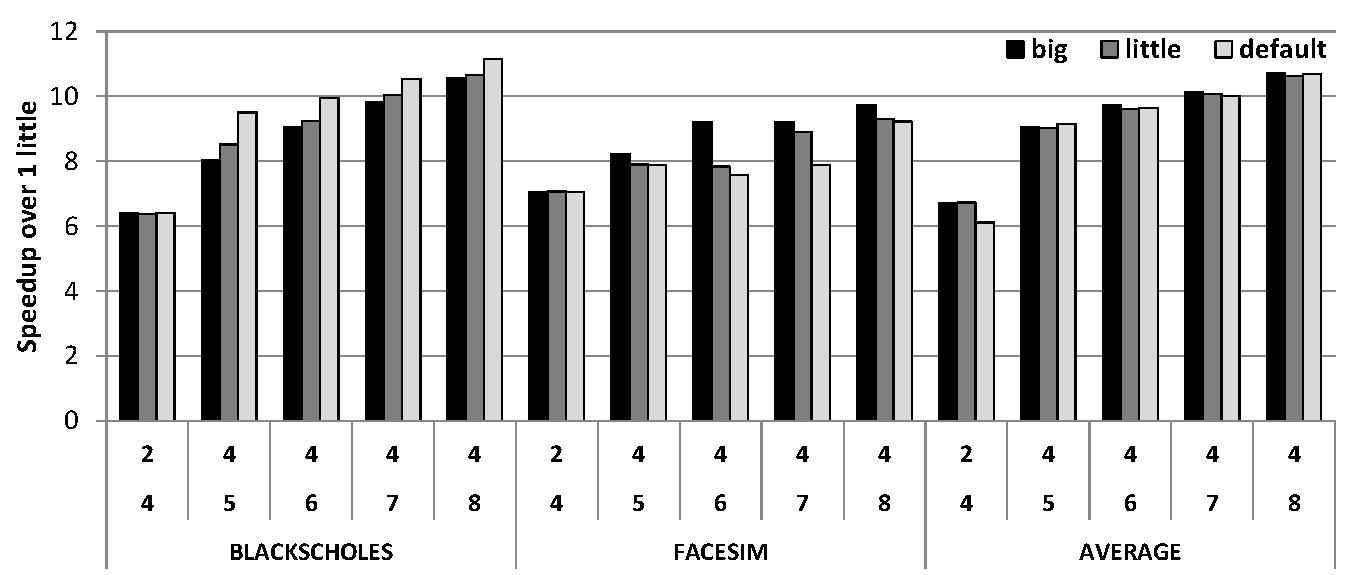
\includegraphics[width=\columnwidth]{figures/speedup-def-big-little}\\%
	\caption{Speedup obtained from the three different scenarios of the main thread's execution. Bottom line numbers show the total number of cores and upper line numbers show the number of big cores.}%
        \label{fig:speedup-def-big-little}%
\end{figure}


Figure~\ref{fig:speedup-def-big-little} shows the obtained speedup from the above scenarios. 
The experiments were conducted on all the nine applications of the evaluation, but we only show results from blackscholes and facesim applications as well as the average speedup of all the applications of this paper.
The blackscholes results clearly indicate that the application does not benefit from the big or little policies.                                                                                                   
When running on 5 cores (\texttt{4+1} configuration), the default policy provides a speedup of 9.5$\times$ while the other two are below 8.3$\times$.                                                                                                               
This application benefits from the default policy where runtime activity takes place on the first available core.
Forcing the runtime to execute on a specific core can lead to increased idle time of the main thread while it is waiting for the specific core to finish with the execution of tasks.

The facesim results show that the migration of the main thread on big provides significant benefits: when running on 6 cores, 4 big and 2 little, the big policy provides a speedup beyond 9$\times$, while the default policy just provides speedup below 8$\times$.
The reason why facesim's behaviour is opposed to the one seen in case of blackscholes relies on the idle time of the big cores.                                                                                                              
The overall scalability of facesim is limited compared to blackscholes: it has frequent barriers followed by short sequential phases. 
By forcing the main thread to execute on a big core, these frequent sequential phases are executed faster which helps to the better utilization of big cores.
%As a result, big cores are not fully-utilized. 
Therefore, it is beneficial to assign the runtime activities to a big core.

%does not get delayed by being restricted to a single big core.     

The average results of all the applications do not provide any significant gain due to the big and little policies since the small speedups observed for some applications are compensated by the small slowdowns seen in some others. In general, the noise introduced by the runtime activity to user tasks in the task-based programming model is reduced. The memory footprint of this activity is very small, as the runtime only accesses some data structures and does not need to buffer large messages as in the case of the MPI runtime. Also, since the task-based runtime is asynchronous and dynamically schedules tasks, it automatically deals with the load imbalance that it creates. Thus, this activity can be executed on the same core as user tasks without degrading the performance of the application.


%The big policy ensures tasks to be created in a high frequency core, 
%but it may happen that this core is busy running user code, 
%which forces runtime activity to wait and, therefore, leaves some cores idle.                               


\iffalse
The OmpSs runtime system can run on any core under its default execution mode.                                                                                                                                                               
Also, runtime activity can migrate from one core to another depending on the hardware state and the need for creating new tasks.                                                                                                             
This implies complex and interesting trade-offs between the runtime system overhead and the tasks execution time.                                                                                                                            
For example, if the runtime system runs on a little core, some tasks                                                                                                                                                                         
will be created under a slow frequency regime but, as a counterpart, tasks will have all the big cores                                                                                                                                      
available to run.                                                                                                                                                                                                                            
Otherwise, if tasks are created in a big core, they will be able to start running before the previous scenario                                                                                                                              
but one of the big cores is not going to be focused on executing user code.                                                                                                                                                                 

While the default runtime system mode is very flexible and makes sure that tasks are created and scheduled whenever there is a free core to perform such operations, it is not clear whether it always constitutes the best possible option. 
In this section, we evaluate two alternative runtime system running policies and we compare them with the default one.                                                                                                                       
The first policy consists in forcing the runtime activity to always run in a big core and the second one forces the runtime to run on a little core.                                                                                        
We allow the cores responsible for the runtime activity to execute user code tasks if there are no runtime operations required.
In this sense, the responsible cores are not exclusively dedicated to the runtime but they can be considered assistant cores since they have the exclusive role of running system software routines, as the other cores will just run application user defined tasks.


In Figure~\ref{fig:speedup-def-big-little} we see an evaluation taking into account the three policies: Default, which consists in letting the runtime to freely execute in all the cores, Big, which consists in forcing the runtime to run in a big core and Little, which
forces the runtime system to run in a little core.                                                                                                                                                                                    
In the left hand side of the figure we show results concerning the BlackScholes application. We consider 5 different execution scenarios, the first one runs the application in 4 cores, 2 small and 2 little, while the other scenarios consider 5 cores (4 big and 1 small), 6 cores (4 big and 2 small), 7 (4 big and 3 small) and 8 (4 big and 4 small).                                                        
                                                                      
The results regarding the BlackScholes application clearly indicate that the application does not benefit from the Big or Little policies.                                                                                                   
When running on 5 cores, 4 big and 1 little, the default policy provides a speedup of 9.5x while the other two are below 8.3x.                                                                                                               
This application benefits from the default policy when tasks are created whenever one core is ready to do so.                                                                                                                                
The Big policy ensures tasks to be created in a high frequency core, but it may happen that this core is busy running user code, which forces runtime activity to wait and, therefore, leaves some cores idle.                               
                                                                                                                                                                                                                                             
Figure~\ref{fig:speedup-def-big-little} also shows results for the Facesim application using the same experimental setup as the one described for BlackScholes. 
In this case, the Big policy provides significant benefits: when running on 6 cores, 4 big and 2 little, the Big policy provides a speedup beyond 9x, while the default policy just provides speedups below 8x.                              
The reason why Facesim's behavior is opposed to the one seen in case of BlackScholes relies on the idle time of the big cores.                                                                                                              
The overall scalability of Facesim is worse than BlackScholes, which implies that the big cores are not utilized as much and, therefore, task creation and scheduling does not get delayed by being restricted to one single big core.     

The average results concerning all the applications do not provide any significant gain due to the big and little policies since the wins observed for some applications are compensated by the losses seen in some others.
\fi